\documentclass[12pt]{article}
\usepackage{frExamplee}
\usepackage{booktabs}       % professional-quality tables
\usepackage{amsfonts}       % blackboard math symbols
\usepackage{amsmath}
\usepackage{enumitem}
\usepackage{listings}
\lstset{
    language=Python,
    basicstyle=\scriptsize\ttfamily,
    keywordstyle=\color{blue},
    commentstyle=\color{green!50!black},
    stringstyle=\color{red},
    showstringspaces=false,
    numbers=left,
    numberstyle=\footnotesize,
    numbersep=5pt,
    frame=single,
    breaklines=true,
    breakatwhitespace=true,
    tabsize=4,
    captionpos=b
}
\usepackage{amssymb}
\usepackage{graphicx}
\usepackage{csquotes}
\usepackage[backend=biber, style=ieee,]{biblatex}
\usepackage{setspace}
\usepackage[usenames, dvipsnames]{xcolor}
\usepackage{xspace}
\usepackage{caption}
\usepackage{subcaption}
\usepackage{multirow}
\usepackage{float}
\usepackage{wrapfig}
\usepackage{placeins}
\usepackage{algpseudocode}
\usepackage{algorithm}
\usepackage{algorithmicx}
\usepackage{hyperref}
\usepackage{setspace}
\usepackage{fancyhdr} 
\fancyhf{}
\cfoot{\thepage}
\pagestyle{fancy}
\renewcommand{\headrulewidth}{0pt}%

\addbibresource{FRtemplates/frExampleRefs.bib}
\title{Exploration of Governing Laws of Blackbody Radiation}
\author{
Tony Wang \href{https://orcid.org/0009-0009-3015-7192}{
\includegraphics[height=12pt]{figure/orcid.png}}\\
\texttt{1009027447 | wangq330} \\
\texttt{tonyivt.wang@mail.utoronto.ca}\\
\And
Rowan Mackintosh \\
\texttt{1009306715 | macki180} \\
\texttt{rowan.mackintosh@mail.utoronto.ca} \\
}
\begin{document}
\maketitle
\begin{abstract}
This lab report investigates the principles of blackbody radiation and explores the spectral distribution of electromagnetic radiation emitted by a blackbody, emphasizing key principles such as Wien's Displacement Law and the Stefan-Boltzmann Law. The experimental setup involves a prism spectrophotometer to measure the intensity of blackbody radiation at various temperatures. Through two experiments, we found Wien's Displacement Constant to be $(1.73 \pm 0.75) \times 10^{-3}\;[m\cdot K]$ and verified the Stefan-Boltzmann Law by confirming the proportionality between intensity and temperature raised to the power of four. Discussions also include the validity of assumptions made and the application of blackbody radiation in the efficiency of incandescent lights.
\end{abstract}

\section{Introduction}
Above absolute zero, objects emit thermal radiation due to the conversion of their thermal energy. The concept of a blackbody, absorbing all radiation and displaying temperature-dependent color, was introduced to explain the spectral distribution observed during heating. This exploration revealed a discrepancy with classical physics, introducing "the ultraviolet catastrophe" that prompted Max Planck to introduce the concept of energy quantization, paving the foundation of quantum mechanics. \autocite{PhysRevLett.42.835}.

Heated objects tend to glow orange and red because the peak of the intensity of blackbody radiation shifts to lower wavelengths (higher energy) as temperature increases. It can be modeled with Wien's Displacement Law \autocite{manuall}:
\begin{equation}
    b=\lambda_{\rm max}T=2.898\times10^{-3}\;[mK]
    \label{eq:wien}
\end{equation} 
where $\lambda_{\rm max}$ and $T$ correspond to the wavelength of the peak and the emitting object's temperature respectively. Similarly, the Stefan-Boltzmann Law reinforces this relationship, modeling the increase of energy emission as temperature increases for a body \autocite{manuall}:
\begin{equation}
    I=\frac{P}{A}=\varepsilon\sigma T^4
    \label{eq:stefan}
\end{equation}
where $P$ is power, $A$ is surface area and $I$ is radiation intensity. $\varepsilon$ is emissivity, where $\varepsilon<1$ symbolizes a grey body, and $\varepsilon=1$ represents a black body. Finally $\sigma=5.67\times10^{-8}\;\left[\frac{W}{m^2K^{4}}\right]$ is the Stefan-Boltzmann constant.

Building on top of these relationships, we also know that blackbody radiation emits as a spectrum, with intensity varying based on frequency or wavelength. The classical Rayleigh-Jeans Law considers cavity atoms as oscillators emitting waves across all wavelengths \autocite{manuall}:
\begin{equation}
    I(\lambda,T)=\frac{dI}{d\lambda d\Omega}=\frac{2\pi ckT}{\lambda^4}
    \label{eq:jeans}
\end{equation}
where $k,\;c$ are Boltzmann's constant and speed of light in a vacuum, respectively. While this approximation works well for long wavelengths, the intensity will approach infinity as lambda becomes small, which is what the "ultraviolet catastrophe" refers to. This led to the derivation of Planck's Radiation Law which compared to (\ref{eq:jeans}), modeled intensity much more accurately \autocite{planck1900theory}:
\begin{equation}
    I(\lambda,T)=\frac{2hc^2}{\lambda^5\exp\left(\frac{hc}{\lambda kT}\right)}
    \label{eq:planck}
\end{equation}
where Planck's constant, $h$, is introduced into the equation. This model is way more consistent with experimental data and it provides a foundational understanding of the spectral distribution of electromagnetic radiation emitted by a blackbody, laying the groundwork for the development of quantum theory and contributing to the formulation of key principles in numerous engineering fields \autocite{PhysRevLett.42.835}.

\section{Experiment}
\begin{figure}[htbp]
\centering
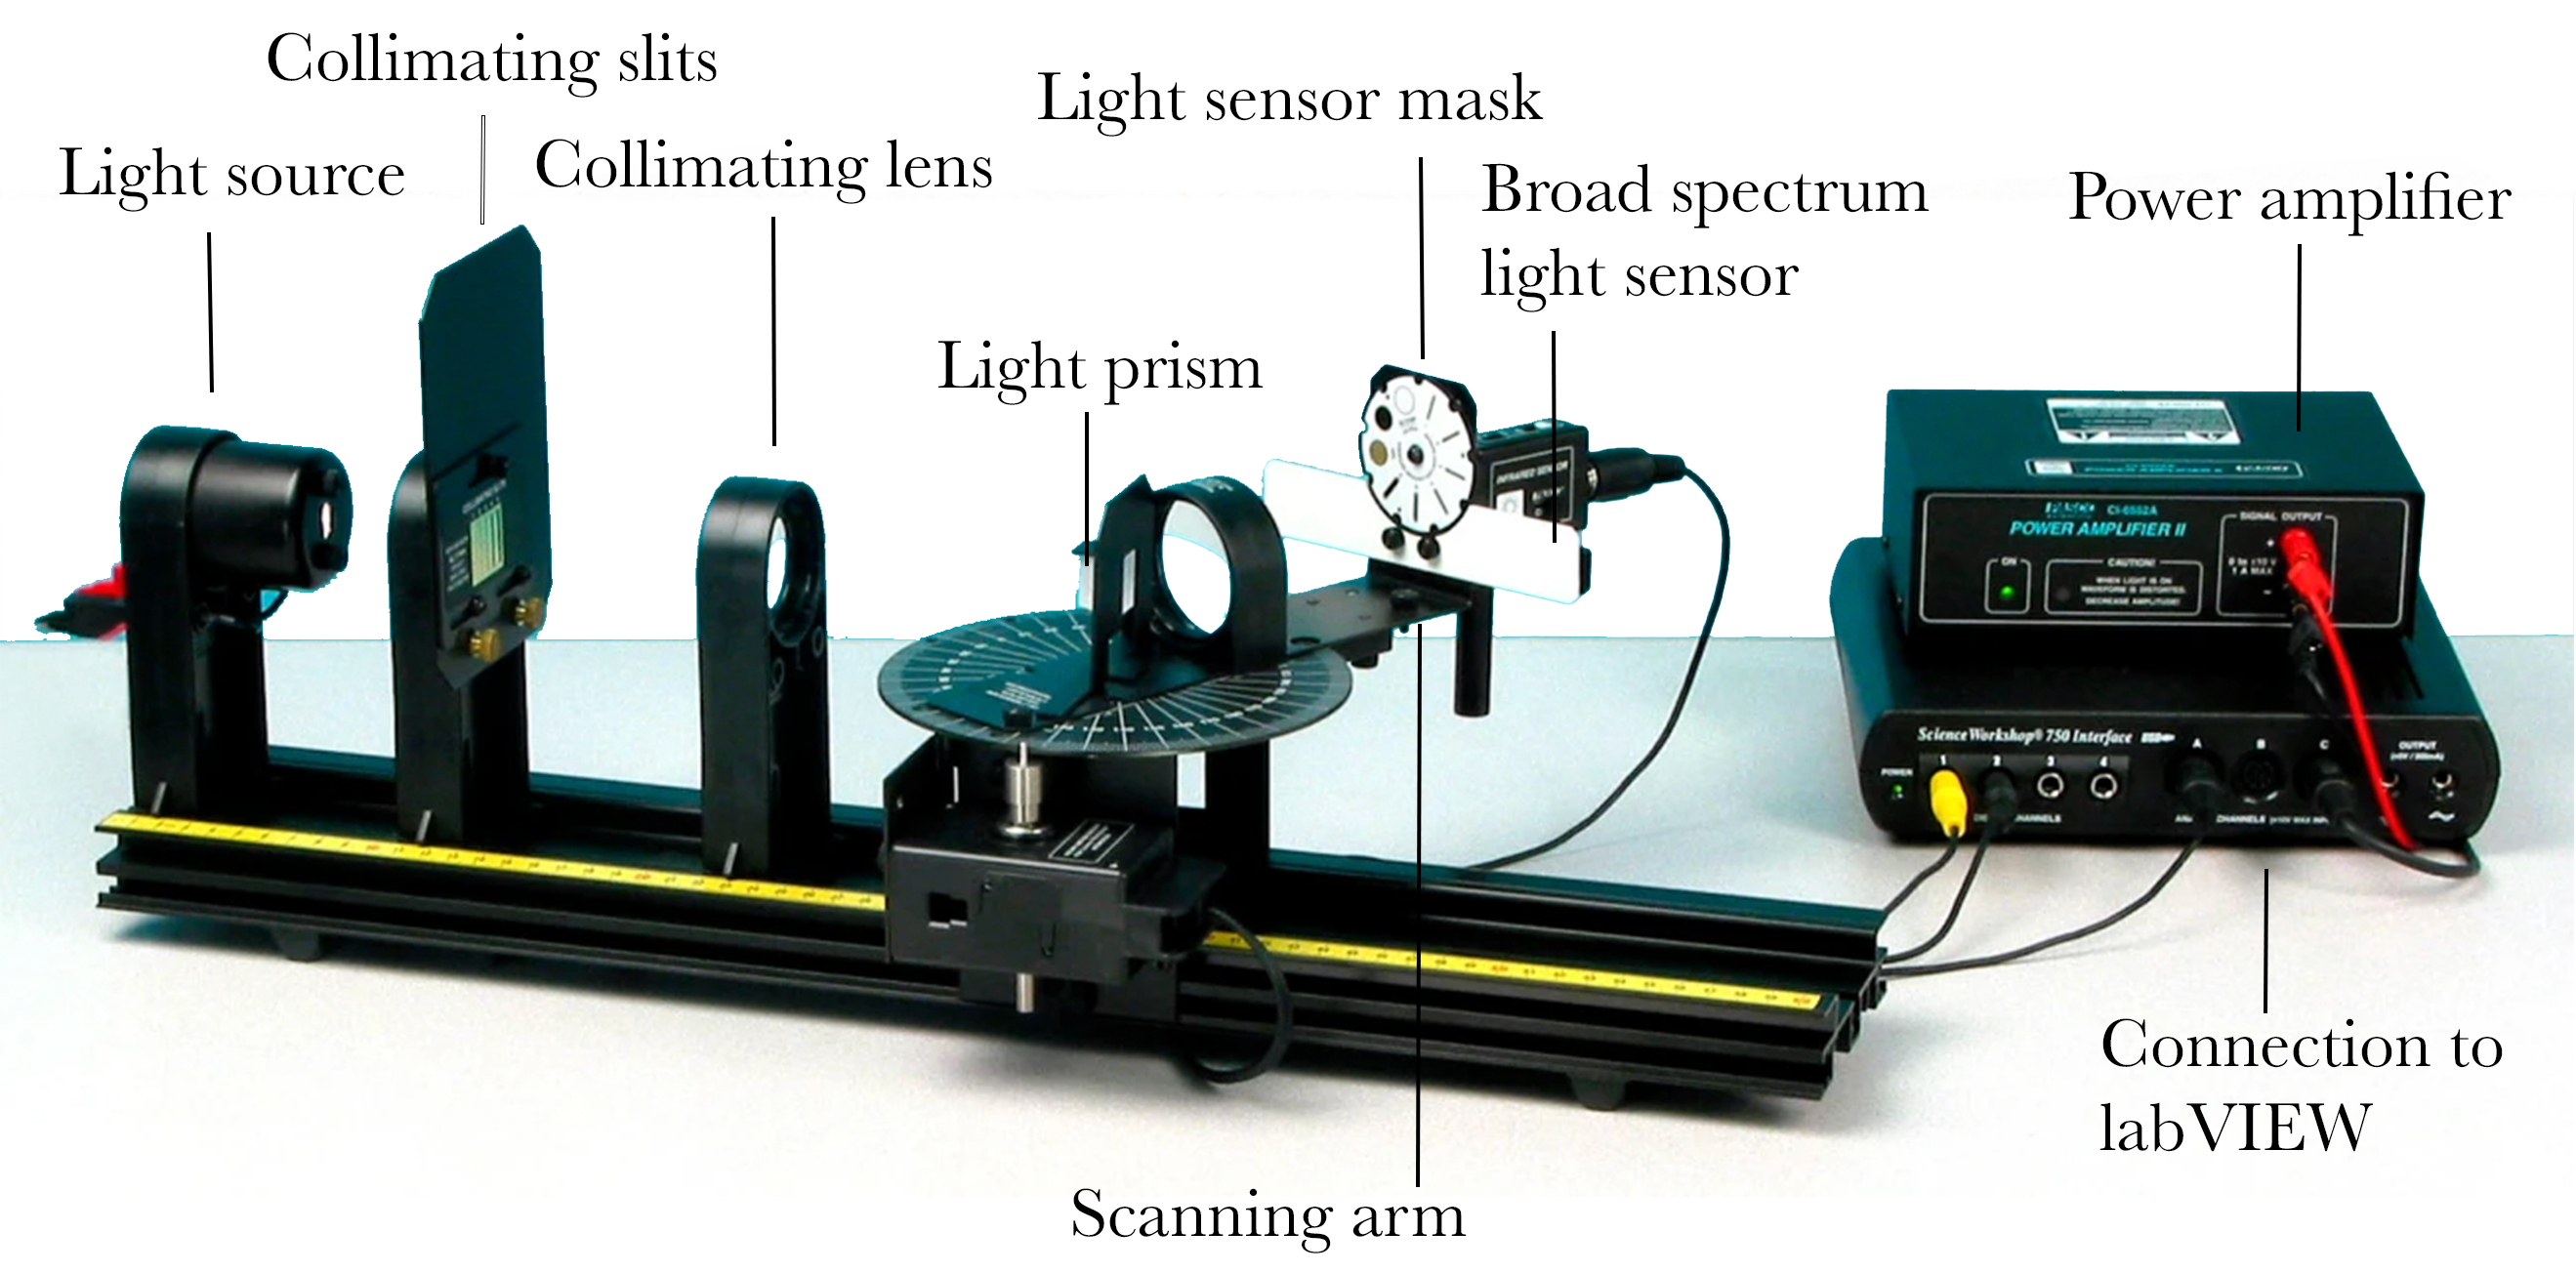
\includegraphics[width=0.875\columnwidth]{figure/aparatus.png}
\caption{Labelled experimental setup \autocite{boyer2018blackbody}.}
\label{fig:aparatus}
\end{figure}

\subsection{Equipment and Uncertainties}
\begin{itemize}
    \item Prism spectrophotometer (subcomponents labeled in Fig. \ref{fig:aparatus})
    \begin{itemize}
        \item Blackbody (incandescent light source)
        \item Collimating slits
        \item Collimating lens
        \item Light prism
        \item Light sensor mask
        \item Broad spectrum light sensor $\big(\pm1\times10^{-5}\;[V]\big)$
        \item Power amplifier
        \item Scanning arm $(\pm0.1^\circ)$
    \end{itemize}
    \item Blackbody radiation LabVIEW
\end{itemize}

\subsection{Method}
The analysis of energy emitted by an incandescent light bulb is conducted using the prism to separate light into wavelengths and the spectrophotometer to measure light intensity based on incident angles. The prism's chromatic dispersion causes different wavelengths to refract by varying amounts. A Broad Spectrum Light Sensor, in conjunction with the prism, facilitates scanning the complete spectrum (approximately 400 nm to 2500 nm). Wavelengths corresponding to angles are calculated using prism spectrophotometer equations (\ref{sec:prism}). This allows for the plotting of relative light intensity against wavelength during the scanning process, resulting in the distinctive blackbody curve. As the power input to the light bulb decreases, both its temperature (\ref{sec:temp}) and light intensity reduces. Repeating this measurement across different temperatures illustrates the shifts in peak wavelength in the curves \autocite{manuall}. We will utilize the angles, wavelengths, and temperatures collected this way to verify Wien's Displacement Law and Stefen-Boltzmann Law (\ref{eq:wien}, \ref{eq:stefan}).

\subsubsection{The light prism: determining wavelengths from angle measurements} \label{sec:prism}
The prism (labeled in Fig. \ref{fig:aparatus}) is mounted such that incident light hits at an angle of $60^\circ$. By applying Snell's Law on the refracting faces of the triangular prism, we deduce the relation for index of refraction:
\begin{equation}
    n(\theta)=\sqrt{\left(\frac{2\sin\theta}{\sqrt{3}}+\frac{1}{2}\right)^2+\frac{3}{4}}
    \label{eq:snell}
\end{equation}
However, $n$ varies with a change in wavelength, $\lambda$, and hence we will need the Caunchy equation \autocite{manuall}:
\begin{equation}
    n(\lambda)=\frac{A}{\lambda^2}+B
    \label{eq:cauchy}
\end{equation}
where $A=13900\;[nm],\;B=1.689$. Combining equations (\ref{eq:snell}, \ref{eq:cauchy}) and subbing in values for the constants, we obtain:
\begin{equation}
    \lambda(\theta)=\left({\frac{13900}{\sqrt{\left(\frac{2\sin\theta}{\sqrt{3}}+\frac{1}{2}\right)^2+\frac{3}{4}}-1.689}}\right)^\frac{1}{2}\;[nm]
    \label{eq:lambda(theta)}
\end{equation}

\subsubsection{Determining blackbody temperature} \label{sec:temp}
We start by relating the electrical resistance of the blackbody (in our case the tungsten filament of the light source, labeled in Fig. \ref{fig:aparatus}) and its temperature \autocite{manuall}:
\begin{equation}
    R=R_0\left[1+\alpha_0(T-T_0)\right]
    \label{eq:resistance}
\end{equation}
where $\alpha_0=4.5\times10^{-3}\;\left[\frac{1}{K}\right]$ is the temperature coefficient at $T_0=293\;[K]$, and $R_0=1.1\;[\Omega]$. And rearranging equation (\ref{eq:resistance}) and using Ohm's Law, we arrive at:
\begin{equation}
    T=T_0+\frac{\frac{V}{IR_0}-1}{\alpha_0}
    \label{eq:temperature}
\end{equation}
where $V,\;I$ are voltage and current, and we will assume the room temperature to not deviate significantly from $20^\circ C$.

\subsection{Experimental Procedure}
\begin{enumerate}
    \item Power on and connect the apparatus as shown in Fig. \ref{fig:aparatus}.
    \item On the physical setup, rotate the scanning arm counterclockwise until the end to reset the position. Set the collimating slits on slit 4, and the light sensor mask on slit 3. Set the broad spectrum light sensor to 'x10' and tare. Place the collimating lens approximately 10 $cm$ away from the collimating slits. The scanning arm should be reset and the tare should be pressed after every trial.
    
    \textbf{Measuring initial angle (\ref{sec:initial})}
    \vspace{-10pt}
    \item On labVIEW, set acquisition to $80^\circ$ and voltage to 6 $V$.
    \item Rotate the scanning arm to start the experiment, record $\theta_{\rm init}$ (the initial angle should be recorded as the angle at which the second peak occurred in the $I-\theta$ plot) and color of light coming from the source. Repeat 5 times.

    \textbf{Wien's Displacement Law (\ref{sec:wien})}
    \vspace{-10pt}
    \item Switch acquisition to $30^\circ$ and voltage to 10 $V$. Rotate the scanning arm to start the experiment, and record $\theta_{\rm peak}$, current, and intensity.
    \item Repeat step 5 three times for each voltage, stepping down 1 $V$ until 4 $V$ inclusive to a total of 21 trials.

    \textbf{Stefan-Boltzmann Law (\ref{sec:stefan})}
    \vspace{-10pt}
    \item Set voltage back to 10 $V$.  Rotate the scanning arm to start the experiment, use labVIEW to find the area under the visualized curve, and record it.
    \item Repeat step 7 five times for each voltage, stepping down 1 $V$ until 4 $V$ inclusive to a total of 35 trials.
\end{enumerate}

\section{Results and Discussion}
\subsection{Measuring Initial Angle} \label{sec:initial}
After five trials, we found the average value of the initial angle to be (see Table \ref{table:initangle}):
\begin{equation}
    \theta_{\rm init}=78.4\pm0.2^\circ.
    \label{eq:init}
\end{equation}
This is reasonably close to $80^\circ$ and the consistency between trials (Fig. \ref{fig:initangle}) suggest the validity of this measurement. 

\begin{figure}[htbp]
\centering
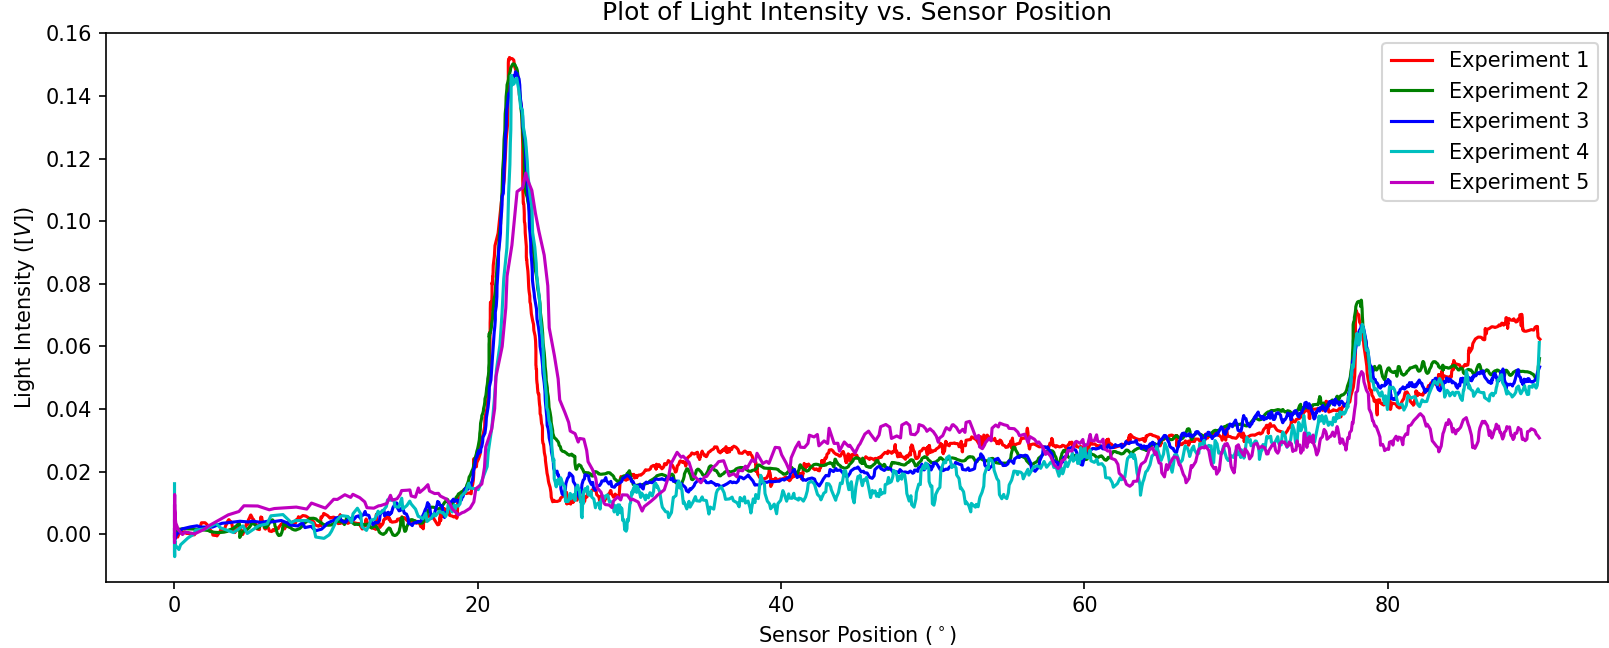
\includegraphics[width=1\columnwidth]{figure/initangle.png}
\caption{Plot of intensity vs. sensor position. Throughout all five trials, the second peak, which is what we will use to estimate $\theta_{\rm init}$, occurs near $80^\circ$.}
\label{fig:initangle}
\end{figure}

In terms of uncertainties, the biggest source of error is the lack of resolution of data, where we are unable to determine precisely where the peak is. While this is directly related to the measurement rate of the labVIEW, the bigger problem lies within the lack of smoothness in the scanning arm. Applying a small moment is not enough to overcome friction and move the arm, yet just a bit too much force will cause it to rotate too quickly, causing resolution to be rough.

\subsection{Wien's Displacement Law} \label{sec:wien}
We aim to experimentally find Wien's Displacement Constant using equation (\ref{eq:wien}) and compare it to the expected value, where we obtain $\lambda_{\rm max}$ from (\ref{eq:lambda(theta)}) and $T$ from (\ref{eq:temperature}) with our measured voltage, current, angle and associated constants. Instead of the raw interpreted angle from the intensity plot, we will use the adjusted angle, $\theta_{\rm adjusted}$ by taking the difference between $\theta_{\rm init}$ (\ref{eq:init}) and the raw angle. With voltage as control, we collected three sets of data for each voltage with seven data points (see Table \ref{table:wien}), where we found the constant to be:
\begin{equation}
    b=(1.73 \pm 0.75) \times 10^{-3}\;[m\cdot K]
    \label{eq:b}
\end{equation}
There is about a 50\% error compared to the expected value, and the real value does not fall within the uncertainty range. This means there are sources of error that we failed to include in our uncertainty propagation. This may include our assumption of the tungsten filament at high temperature inside the light source to be a perfect blackbody, which is a reasonable approximation since the spectral distribution of emitted radiation is close to that of a blackbody, but we are unable to acquire the error in this department \autocite{10.1119/1.4802873}. The uncertainty of $V$ and $I$ measured through labVIEW may also be higher than the significant figures they provide, although we have no way of knowing their precise values. Finally, the errors related to manually rotating the scanning arm and the roughness of angle data discussed in \ref{sec:initial} are also significant.

\subsection{Stefan-Boltzmann Law} \label{sec:stefan}
\begin{figure}[htbp]
\centering
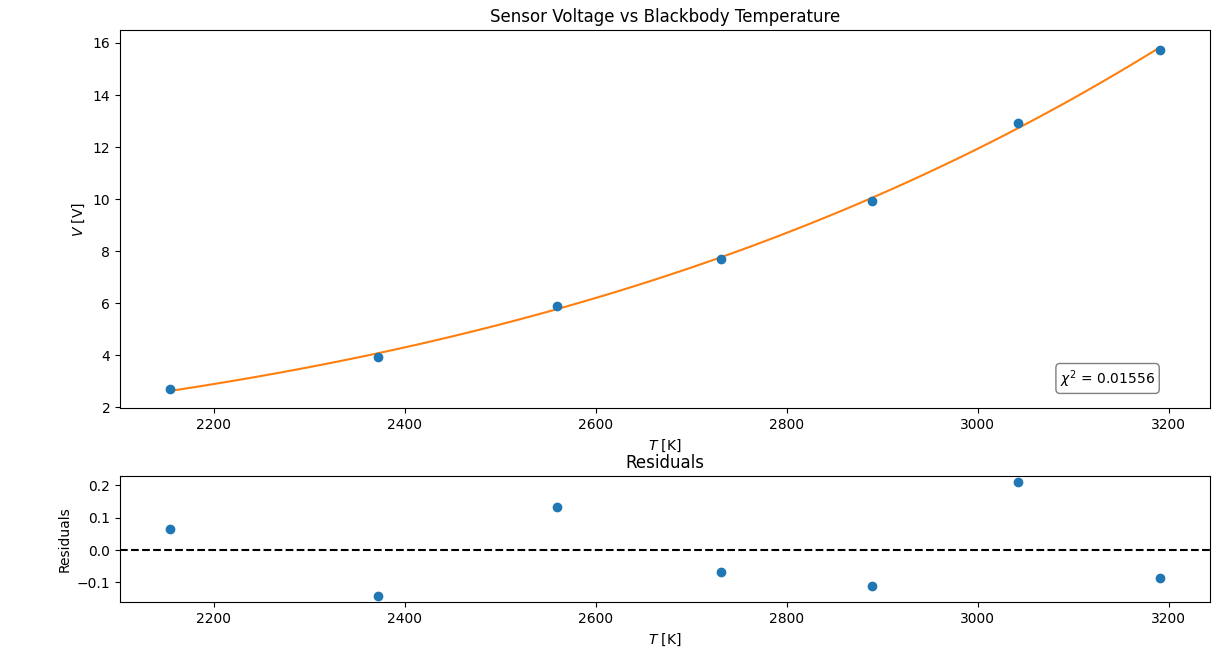
\includegraphics[width=1\columnwidth]{figure/stefan.png}
\caption{Plot of average sensor voltage vs. average blackbody temperature fitted with a power function.  Uncertainty bars were plotted in both the x and y axes but are too small to be seen, see specific values in Table \ref{tab:stefan}. Regular $\chi^2$ and uncertainty of the power fitted was calculated via a python script (see sec. \ref{sec:python}) with scipy \autocite{2020SciPy-NMeth}. The value and critical value are found to be $\chi^2=0.01556,\;\chi^2_{0.5,49}=1.600$ respectively.}
\label{fig:stefan}
\end{figure}

According to the Stefan-Boltzmann Law (\ref{eq:stefan}), intensity is proportional to temperature raised to the power of four via the product of two constants, emissivity and the Stefan-Boltzmann Constant. To test the principle, we aim to plot our intensity, the average sensor voltage found by numerical integration of the $I-\theta$ curve, against $T$, found with equation (\ref{eq:temperature}) and fit a power function (Fig. \ref{fig:stefan}). 
The fitted function turned out to be:
\begin{equation}
    V=0.000\cdot T^{4.59\pm0.74}+0.0276\pm0.0410
    \label{eq:stefanfit}
\end{equation}
While the power we managed to fit was not precisely 4, 4 does lie within the uncertainty range propagated for the exponent, demonstrating that the proportionality of $I$ and $T^4$ in the Stefan-Boltzmann Law is indeed valid. Based on the $\chi^2$ test, we found the $\chi^2$ value to be very small (0.01556) and less than the critical value (1.600), symbolizing a statistically precise fit and that datapoint uncertainties are negligible. Also taking a look at the residuals plot, all the residuals are small and scatter evenly along 0 with no sign of heteroscedasticity, also suggesting a good fit. Moreover, the y-intercept is small and experimentally zero considering uncertainties, suggesting that our trends also match well to that of (\ref{eq:stefan}) where intensity should be 0 and 0 $K$. However, we recognize that the uncertainties of this regression fit are relatively large, and that is mainly attributed to us fitting to higher exponents and that parameters are highly sensitive, as our datapoint uncertainties are nearly negligible as analyzed prior. It should also be commented on that the determination of uncertainty for the average sensor voltage (found through numerical integration of the $I-\theta$ curve) may not be precise, as it relies heavily on human judgment and errors are hard to quantify. For instance, there will be uncertainty in how precise the measurement of the angle is, the resolution of data or sampling rate, and human error. Depending on what we set these uncertainties to, the propagated uncertainties, especially the fitting uncertainties will vary greatly.

\subsection{Analyzing the Blackbody Light Source}
After turning on the light source (the blackbody), it started yellow and red and became progressively whiter as the temperature increased. This can be explained with Planck's Radiation Law (\ref{eq:planck}), where as temperature increase intensity will peak at a shorter wavelength (Yellow and red has the longest wavelengths in the visible spectrum, when the peak happens at a shorter wavelength more parts of the visible spectrum is included, and a full spectrum produces white light \autocite{Eberly:77}. See Fig. \ref{fig:curves} for visual aid of this trend) \autocite{manuall}. 

\begin{figure}[htbp]
\centering
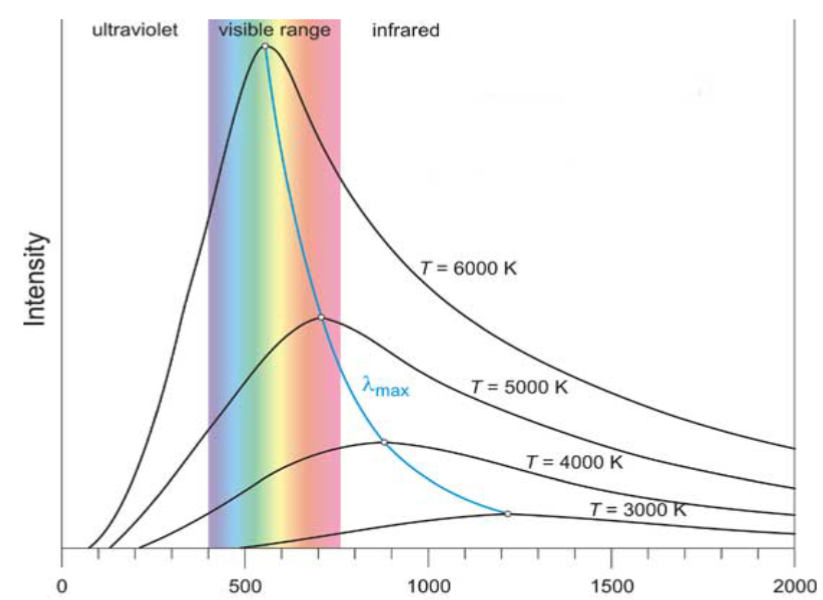
\includegraphics[width=0.5\columnwidth]{figure/curves.png}
\caption{$I-\lambda$ curves at different temperatures \autocite{curves} for a blackbody. As temperature increases, the intensity curves will peak at a shorter wavelength.}
\label{fig:curves}
\end{figure}

Upon rotating the scanning arm after the light warms up, the full visible spectrum was visible on the light sensor screen. The rainbow on the sensor also becomes brighter as the light source became brighter due to the same reason, where especially the blue and violet regions were more visible due to the same reason explained above. In Fig. \ref{fig:curves}, we can clearly see that at the highest temperature, the peak will be in the visible range, and as the temperature starts low it will be in the infrared range. To make our lightbulb more efficient, that is to say, more wavelengths are emitted in the visible spectrum, we should make sure the operating temperature is high enough such that the peak is in the visible range. We can also apply emissivity coatings to enhance the emission of light \autocite{curves}.

\section{Conclusion}
In conclusion, this laboratory experiment successfully explored and verified key principles related to blackbody radiation. The determination of the initial angle, $\theta_{\rm init}$, demonstrated reasonable consistency and accuracy, validating the reliability of the experimental measurements. However, the experimental determination of Wien's Displacement Constant yielded a result with a significant deviation from the expected value, $b=(1.73 \pm 0.75) \times 10^{-3}\;[m\cdot K]$ versus the real value, $b=2.898\times10^{-3}\;[m\cdot K]$, indicating potential sources of error and the need for further investigation. Possible errors include assumptions about the blackbody nature of the tungsten filament, uncertainties in voltage and current measurements, and challenges in the smooth rotation of the scanning arm.

On the other hand, the experimental verification of the Stefan-Boltzmann Law showed a strong correlation between the intensity and temperature, supporting the proportionality of $T^4$ in the law, where we were able to fit to a power of $T^{4.59\pm0.74}$. The fitting of the power function provided a close match to the theoretical expectations, though the uncertainties in the fitting parameters were relatively large.

The analysis of the blackbody light source's behavior confirmed the theoretical predictions based on Planck's Radiation Law, showcasing the shift in intensity peaks towards shorter wavelengths as temperature increased. Practical considerations for improving the efficiency of light sources were also discussed.

In summary, while the experiment provided valuable insights into blackbody radiation, it also highlighted the importance of addressing potential sources of error for more accurate results. Future work could involve refining experimental techniques, incorporating advanced instrumentation, and exploring additional factors influencing blackbody radiation. The study contributes to a deeper understanding of fundamental principles in physics and their applications in real-world scenarios.

\newpage
\printbibliography

\section*{Appendix}
\subsection*{Tables}
\begin{table}[htbp]
    \centering
    \vspace{10pt}
          \begin{tabular}{cc}
            \hline
            \textbf{Trial} & \textbf{$\theta_{\rm init}\pm0.2\;[^\circ]$} \\
            \hline
            1 & 78.3 \\
            2 & 78.5 \\
            3 & 78.3 \\
            4 & 78.4 \\
            5 & 78.6 \\
            \hline
            Avg & 78.4\\
            \hline
          \end{tabular}
      \caption{Initial angle recorded throughout five trials.}
      \label{table:initangle}
\end{table}

\begin{table}[htbp]
    \centering
    \vspace{10pt}
    \begin{tabular}{cccccc}
        \toprule
        $\theta_{\rm adjusted}$ & $V$ & $I$ & $\lambda_{\text{max}}\;[nm]$ & $T$\;[K]& $B\;[m\cdot K]$\\
        $\pm0.2\;[^\circ]$&$\pm0.5\;[V]$&$\pm0.0005\;[A]$& & & &\\
        \midrule
        $55.9$ & $10$ & $0.649$ & $64.10 \pm 2.75$ & $3183 \pm 1.56 \times 10^{-4}$ & $(2.04 \pm 0.16) \times 10^{-3}$ \\
        $56.1$ & $10$ & $0.646$ & $64.08 \pm 2.75$ & $3198 \pm 1.56 \times 10^{-4}$ & $(2.05 \pm 0.16) \times 10^{-3}$ \\
        $56.0$ & $10$ & $0.648$ & $64.09 \pm 2.75$ & $3190 \pm 1.56 \times 10^{-4}$ & $(2.04 \pm 0.16) \times 10^{-3}$ \\
        $56.1$ & $9$ & $0.611$ & $64.08 \pm 2.75$ & $3046 \pm 1.65 \times 10^{-4}$ & $(1.95 \pm 0.17) \times 10^{-3}$ \\
        $55.9$ & $9$ & $0.613$ & $64.10 \pm 2.75$ & $3036 \pm 1.65 \times 10^{-4}$ & $(1.95 \pm 0.17) \times 10^{-3}$ \\
        $56.0$ & $9$ & $0.612$ & $64.09 \pm 2.75$ & $3041 \pm 1.65 \times 10^{-4}$ & $(1.95 \pm 0.17) \times 10^{-3}$ \\
        $55.9$ & $8$ & $0.576$ & $64.10 \pm 2.75$ & $2876 \pm 1.75 \times 10^{-4}$ & $(1.84 \pm 0.18) \times 10^{-3}$ \\
        $55.9$ & $8$ & $0.571$ & $64.10 \pm 2.75$ & $2901 \pm 1.77 \times 10^{-4}$ & $(1.86 \pm 0.18) \times 10^{-3}$ \\
        $55.9$ & $8$ & $0.574$ & $64.10 \pm 2.75$ & $2888 \pm 1.76 \times 10^{-4}$ & $(1.85 \pm 0.18) \times 10^{-3}$ \\
        $55.9$ & $7$ & $0.533$ & $64.10 \pm 2.75$ & $2723 \pm 1.90 \times 10^{-4}$ & $(1.75 \pm 0.19) \times 10^{-3}$ \\
        $55.9$ & $7$ & $0.530$ & $64.10 \pm 2.75$ & $2738 \pm 1.91 \times 10^{-4}$ & $(1.76 \pm 0.19) \times 10^{-3}$ \\
        $55.9$ & $7$ & $0.532$ & $64.10 \pm 2.75$ & $2731 \pm 1.90 \times 10^{-4}$ & $(1.75 \pm 0.19) \times 10^{-3}$ \\
        $56.0$ & $6$ & $0.488$ & $64.09 \pm 2.75$ & $2554 \pm 2.07 \times 10^{-4}$ & $(1.64 \pm 0.21) \times 10^{-3}$ \\
        $56.0$ & $6$ & $0.486$ & $64.09 \pm 2.75$ & $2564 \pm 2.08 \times 10^{-4}$ & $(1.64 \pm 0.21) \times 10^{-3}$ \\
        $56.0$ & $6$ & $0.487$ & $64.09 \pm 2.75$ & $2559 \pm 2.07 \times 10^{-4}$ & $(1.64 \pm 0.21) \times 10^{-3}$ \\
        $55.9$ & $5$ & $0.437$ & $64.10 \pm 2.75$ & $2382 \pm 2.31 \times 10^{-4}$ & $(1.53 \pm 0.23) \times 10^{-3}$ \\
        $55.9$ & $5$ & $0.441$ & $64.10 \pm 2.75$ & $2361 \pm 2.29 \times 10^{-4}$ & $(1.51 \pm 0.23) \times 10^{-3}$ \\
        $55.9$ & $5$ & $0.439$ & $64.10 \pm 2.75$ & $2371 \pm 2.30 \times 10^{-4}$ & $(1.52 \pm 0.23) \times 10^{-3}$ \\
        $55.7$ & $4$ & $0.388$ & $64.12 \pm 2.76$ & $2153 \pm 2.60 \times 10^{-4}$ & $(1.38 \pm 0.26) \times 10^{-3}$ \\
        $55.7$ & $4$ & $0.388$ & $64.12 \pm 2.76$ & $2153 \pm 2.60 \times 10^{-4}$ & $(1.38 \pm 0.26) \times 10^{-3}$ \\
        $55.7$ & $4$ & $0.388$ & $64.12 \pm 2.76$ & $2153 \pm 2.60 \times 10^{-4}$ & $(1.38 \pm 0.26) \times 10^{-3}$ \\
        \midrule
        Avg & - & - & - & -  & $(1.73 \pm 0.75) \times 10^{-3}$ \\
        \bottomrule
    \end{tabular}
      \caption{Calculated data for Wien's Displacement Constant. For uncertainty propagation, see sec. \ref{sec:unc}.}
      \label{table:wien}
\end{table}

\begin{table}[]
    \centering
\begin{tabular}{cc}
\hline
Average Bulb Temperature (K) & Average Sensor Voltage (V) \\
\hline
$3190 \pm 0.00019$ & $15.735 \pm 0.0005$ \\
$3041 \pm 0.00017$ & $12.921 \pm 0.0005$ \\
$2888 \pm 0.00016$ & $9.926 \pm 0.0005$ \\
$2731 \pm 0.00015$ & $7.702 \pm 0.0005$ \\
$2559 \pm 0.00013$ & $5.909 \pm 0.0005$ \\
$2371 \pm 0.00013$ & $3.936 \pm 0.0005$ \\
$2153 \pm 0.00012$ & $2.695 \pm 0.0005$ \\
\hline
\end{tabular}
    \caption{Plotted data points to determine validity of Stefan-Boltzmann Law. For uncertainty propagation, see sec. \ref{sec:unc}.}
    \label{tab:stefan}
\end{table}

\newpage
\subsection*{Uncertainty Propagation} \label{sec:unc}
For equation (\ref{eq:snell}):
\[
\sigma_{n(\theta)}=\frac{\left(\frac{2\sin\theta}{\sqrt3}+\frac{1}{2}\right)\cdot\left(\frac{2}{\sqrt3}\cos\theta\right)}{n(\theta)}\cdot\sigma_\theta
\]
For equation (\ref{eq:lambda(theta)}):
\[
\sigma_\lambda=\frac{\lambda}{2}\cdot \frac{\sigma_{n(\theta)}}{n(\theta)-1.689}
\]
For equation (\ref{eq:temperature}):
\[
\sigma_T=\frac{V}{IR\alpha_0}\cdot\sqrt{\left(\frac{\sigma_V}{V}\right)^2+\left(\frac{\sigma_I}{I}\right)^2}
\]
For equation (\ref{eq:wien}):
\[
\sigma_b=\lambda T\cdot\sqrt{\left(\frac{\sigma_\lambda}{\lambda}\right)^2+\left(\frac{\sigma_T}{T}\right)^2}
\]
\newpage
\subsection*{Plotting and Goodness of Fit Propagation Script} \label{sec:python}
\begin{lstlisting}
import matplotlib.pyplot as plt
import numpy as np
from scipy.optimize import curve_fit
from scipy.stats import chisquare

temperature = [3190.781, 3041.663, 2888.845, 2731.439, 2559.733, 2371.691, 2153.46]
temperature_uncertainty = [0.00019, 0.00017, 0.00016, 0.00015, 0.00013, 0.00013, 0.00012]
voltage = [15.735, 12.921, 9.926, 7.702, 5.909, 3.936, 2.695]
voltage_uncertainty = [0.0005, 0.0005, 0.0005, 0.0005, 0.0005, 0.0005, 0.0005]

def fit_function(T, a, b, c):
    return a * T**c + b

params, covariance = curve_fit(fit_function, temperature, voltage, maxfev=10000)

fig, (ax1, ax2) = plt.subplots(2, 1, figsize=(8, 8), gridspec_kw={'height_ratios': [3, 1]})

ax1.errorbar(temperature, voltage, xerr=temperature_uncertainty, yerr=voltage_uncertainty, fmt='o', label='Data')
T_fit = np.linspace(min(temperature), max(temperature), 100)
V_fit = fit_function(T_fit, *params)
ax1.plot(T_fit, V_fit, label=f'Fit: ${params[0]:.5f} \cdot T^{{{params[2]:.2f}}} + {params[1]:.5f}$')
ax1.set_xlabel('$T$ [K]')
ax1.set_ylabel('$V$ [V]')
ax1.set_title('Sensor Voltage vs Blackbody Temperature')

residuals = voltage - fit_function(np.array(temperature), *params)
ax2.errorbar(temperature, residuals, yerr=voltage_uncertainty, fmt='o')
ax2.axhline(0, color='black', linestyle='--')
ax2.set_xlabel('$T$ [K]')
ax2.set_ylabel('Residuals')
ax2.set_title('Residuals')

chisq_value, _ = chisquare(voltage, fit_function(np.array(temperature), *params))

ax1.text(0.95, 0.05, f'$\chi^2$ = {chisq_value:.5f}', transform=ax1.transAxes, ha='right', va='bottom', bbox=dict(boxstyle='round', facecolor='white', alpha=0.5))

plt.tight_layout()
plt.show()

\end{lstlisting}
\end{document}